\documentclass{article}
\usepackage[utf8]{inputenc}
\usepackage[english]{babel}
\usepackage[]{amsthm} %lets us use \begin{proof}
\usepackage[]{amssymb} %gives us the character \varnothing
\usepackage[margin=0.75in]{geometry}
\usepackage{amsmath}
\usepackage{graphicx}
\usepackage{derivative}
\usepackage{booktabs}
\usepackage[dvipsnames]{xcolor}
\usepackage{comment}
\usepackage{fancyhdr}
\usepackage{breqn}
\usepackage{float}
\usepackage[shortlabels]{enumitem}
\graphicspath{ {./images/} }

\title{ECON 6090-Microeconomic Theory. TA Section 4}
\author{Omar Andujar}
\date{\today}
%This information doesn't actually show up on your document unless you use the maketitle command below

\begin{document}
\raggedright
\pagestyle{fancy}
\fancyhf{}
%\fancyhead[R]{Omar Andujar}
%\fancyhead[L]{Homework 5}
%\fancyfoot[L]{\hrule Some of the problems were discussed with }

\maketitle %This command prints the title based on the information entered above

\section*{In Section notes}
Assumptions
\begin{enumerate}
    \item $u(.)$ represents $\succsim$ and is continuous.
    \item $\succsim$ satisfies local non satiation. (LNS)
    \item $\succsim$ is strictly convex.
\end{enumerate}

Expenditure minimization problem (EMP)
\[\min_x p \cdot x \text{ such that } u(x) \geq \bar{u}\]
Hicksian demand: $h(p,\bar{u})$
\begin{enumerate}
    \item If $\inf u(x) \leq \bar{u} \leq \sup u(x)$ then there exist $h^*$ that solves the EMP. (Extreme Value Theorem)
    \item $h(p,\bar{u})$ is homogeneous of degree 0 (HoD0) in price (p).
    \item $u(h(p,\bar{u})) = \bar{u}$. (LNS)
    \item $h(p,\bar{u})$ is a  well-defined function and it is continuous. ($\succsim$ strictly convex $+$ Berge's Theorem of the Maximum)
\end{enumerate}
Expenditure function: $e(p,\bar{u})$
\begin{enumerate}
    \item Continuous in $(p,\bar{u})$.
    \item Nondecreasing in p and strinctly increasing in $\bar{u}$.
    \item HoD 1 in p.
    \item Concave in p.
\end{enumerate}
Roadmap
  \begin{figure}[H]
    \centering
    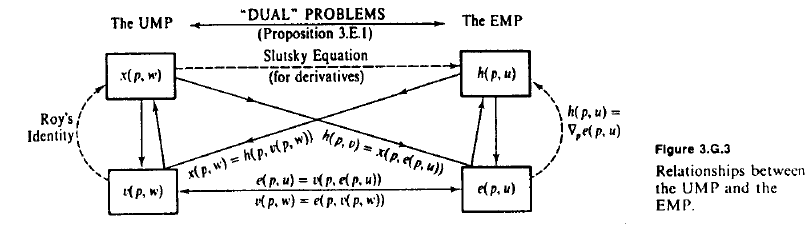
\includegraphics{mwg_chapter3_duality.png}
    \caption{MWG chapter 3. Roadmap.}
    \label{fig:roadmap}
\end{figure}
\section*{Exercises}
\subsection*{(2009 Prelim 1)}
\begin{enumerate}[(a)]
    \item 
    \[\max_{x_1,x_2,x_3} x_1 x_2^{\frac{1}{2}} x_3^{\frac{1}{2}}\]
    Subject to
    \[p_1x_1 +p_2x_2 +p_3x_3 \leq w\]

    \item 
    To find the consumer's demand functions we first notice that $u(.)$ is increasing in each good, so it satisfies LNS and therefore the constraint must be binding. Since all monotonic transformations preserve the order of $\succsim$, solving the problem in $(a)$ is equivalent to,
    \[\max_{x_1,x_2,x_3} log(x_1) + \frac{1}{2}log(x_2)+\frac{1}{2}log(x_3)\]
    Subject to
    \[p_1x_1 +p_2x_2 +p_3x_3 = w\]
    Our Lagrangian is,
    \[\mathcal{L}(x,\lambda) = log(x_1) + \frac{1}{2}log(x_2)+\frac{1}{2}log(x_3) + \lambda(w-p_1x_1 -p_2x_2 -p_3x_3)\]
    And our first order conditions give,
    \[\frac{\partial\mathcal{L}(x,\lambda)}{\partial x_1} = \frac{1}{x_1} - \lambda p_1 = 0\]
    \[\frac{\partial\mathcal{L}(x,\lambda)}{\partial x_2} = \frac{1}{2x_2} - \lambda p_2 = 0\]
    \[\frac{\partial\mathcal{L}(x,\lambda)}{\partial x_3} = \frac{1}{2x_3} - \lambda p_3 = 0\]
    \[\frac{\partial\mathcal{L}(x,\lambda)}{\partial \lambda} = w-p_1x_1 -p_2x_2 -p_3x_3 = 0\]
    From here we obtain,
    \[x_2 = \frac{p_1}{p_2}\frac{x_1}{2}\]
    \[x_3 = \frac{p_1}{p_3}\frac{x_1}{2}\]
    Substituting in the budget constraint,
    \[w = p_1 x_1 + \frac{p_1 x_1}{2} + \frac{p_1 x_1}{2}\]
    Solving the system of equations we get,
    \[\implies x_1(p,w) = \frac{w}{2p_1}\]
    \[\implies x_2(p,w) = \frac{w}{4p_2}\]
    \[\implies x_1(p,w) = \frac{w}{4p_3}\]
    To confirm that these are indeed our walrasian demand functions, we can check the corner solution or compute the Hessian of $u(x)$ and see if it is negative semidefinite.\\
    Since neither of $x_1,x_2,x_3$ equals 0, then the answer above is the Walrasian Demand.

    \item 
    With the addition of the coupon component, the problem becomes,
        \[\max_{x_1,x_2,x_3} x_1 x_2^{\frac{1}{2}} x_3^{\frac{1}{2}}\]
    Subject to
    \[p_1x_1 +p_2x_2 +p_3x_3 \leq w \text{ (Budget constraint)}\]
    \[x_1+x_2+x_3 \leq c \text{ (Coupon constraint)}\]

    \item 
    Yes, for c big enough. Assume $p = (1,1,1)$, and $c>w$, then the problem becomes 
            \[\max_{x_1,x_2,x_3} x_1 x_2^{\frac{1}{2}} x_3^{\frac{1}{2}}\]
    Subject to
    \[x_1 +x_2 +x_3 \leq w \text{ (Budget constraint)}\]
    \[x_1+x_2+x_3 < c \text{ (Coupon constraint)}\]
    The leftover coupons will be $c-w$.
    \item 
    Since the budget constraint and coupon constraint are "parallel", if $c>w$, then we only need to use the budget constraint. Otherwise, if $c \leq w$, we use the coupon constraint.\\
    For example, if $c>w$, we just need to replace $p = (1,1,1)$ in the Walrasian demand we found in $(a)$.
\end{enumerate}

\subsection*{(2023 Prelim 1)}

\begin{enumerate}[(a)]
    \item The problem is
    \[V(T) = \max_{e}B(e) \text{ subject to } \sum_{i=1}^n e_i = T\]
    Let $T_2 > T_1$. Denote $e(T_1)$ as the maximizer under $T_1$. Then there exist $0<\epsilon<\frac{T_2-T_1}{n}$ such that $\sum_{i=1}^n (e_i+\epsilon) = T_1 + n\epsilon < T_2$. Since B is strictly increasing,
    \[B(e+\epsilon) > B(e(T_1))\]
    Also since $\sum_{i=1}^n (e_i+\epsilon) < T_2$,
    \[V(T_2) \geq B(e+\epsilon) >B(e(T_1)) = V(T_1)\]

    \item The problem is
    \[V(T) = \max_{e}B(e) \text{ subject to } \sum_{i=1}^n e_i = T\]
    Since all the conditions are met, we can use the lagrangian method to solve this problem. The lagrangian is,
    \[\mathcal{L} = B(e) + \lambda(T-\sum_{i=1}^n e_i)\]
    And the first order condition is,
    \[\frac{\partial\mathcal{L}}{\partial e_i} = \frac{\partial B(e)}{\partial e_i} - \lambda = 0 \implies \frac{\partial B(e)}{\partial e_i} = \lambda^*\]
    In optimal, by the Envelope Theorem,
    \[\frac{dV(T)}{dT} = \frac{d\mathcal{L}(e^*(T))}{dT} = \lambda^* = \frac{\partial B(e)}{\partial e_i} \]

    \item The problem is
        \[V(T) = \max_{e}b_1(\alpha e_1) + b_2(e_2) \text{ subject to } e_1 + e_2 = T\]
        \[\implies \max_{e_1 \geq 0} b_1(\alpha e_1) + b_2(T-e_1)\]
    The first order condition gives,
    \[\alpha b_1'(\alpha e_1^*(\alpha)) - b_2'(T-e_1^*(\alpha)) = 0\]
    We want to know how does $e_1^*$ changes when a decrease from 1 to $\alpha$ happens. For this we compute the derivative with respect to $\alpha$ on the FOC,
    \[b_1'(\alpha e_1^*(\alpha)) + \alpha b_1''(\alpha e_1^*(\alpha))(e_1^*(\alpha)+\alpha e_1^{*'}(\alpha)) + b_2''(T-e_1^*(\alpha))e_1^{*'}(\alpha) = 0\]
    We group terms and get,
    \[\frac{\partial e_1^*(\alpha)}{\partial \alpha} = -\frac{b_1'(\alpha e_1^*(\alpha)) + \alpha b_1''(\alpha e_1^*(\alpha))e_1^*(\alpha) }{\alpha^2 b_1''(\alpha e_1^*(\alpha)) + b_2''(T-e_1^*(\alpha))}\]
    Since each $b_i$ is strictly increasing and strictly concave, we know $b'(.) >0$ and $b''(.)<0$. From here we obtain that the denominator of $\frac{\partial e_1^*(\alpha)}{\partial \alpha}$ must be negative, but the sign of the numerator, $b_1'(\alpha e_1^*(\alpha)) + \alpha b_1''(\alpha e_1^*(\alpha))e_1^*(\alpha)$, remains undetermined. Therefore the sign of $\frac{\partial e_1^*(\alpha)}{\partial \alpha}$ is undetermined. 

    
\end{enumerate}




\end{document}

